\section{Overview}
\index{Overview}

What is a WebBrick? It is a network connected control and automation product designed around the principle 
of 'local control - global intelligence'. This means that most of the time control is handled locally but a 
system as a whole can be made more intelligent through the use of some central control
(for example the WebBrick Gateway) that provides the global intelligence. i.e. Lights for a room are a local issue, 
but heating is more of an overall control issue. This also means that you are
not dependant on a single control system for the complete system, you can always switch on the lights 
in this room while someone is making changes to a global control system.

Control can be done through a WebBrick's web interface, through its physical inputs or using remote commands.

\begin{figure}[H]
\centering
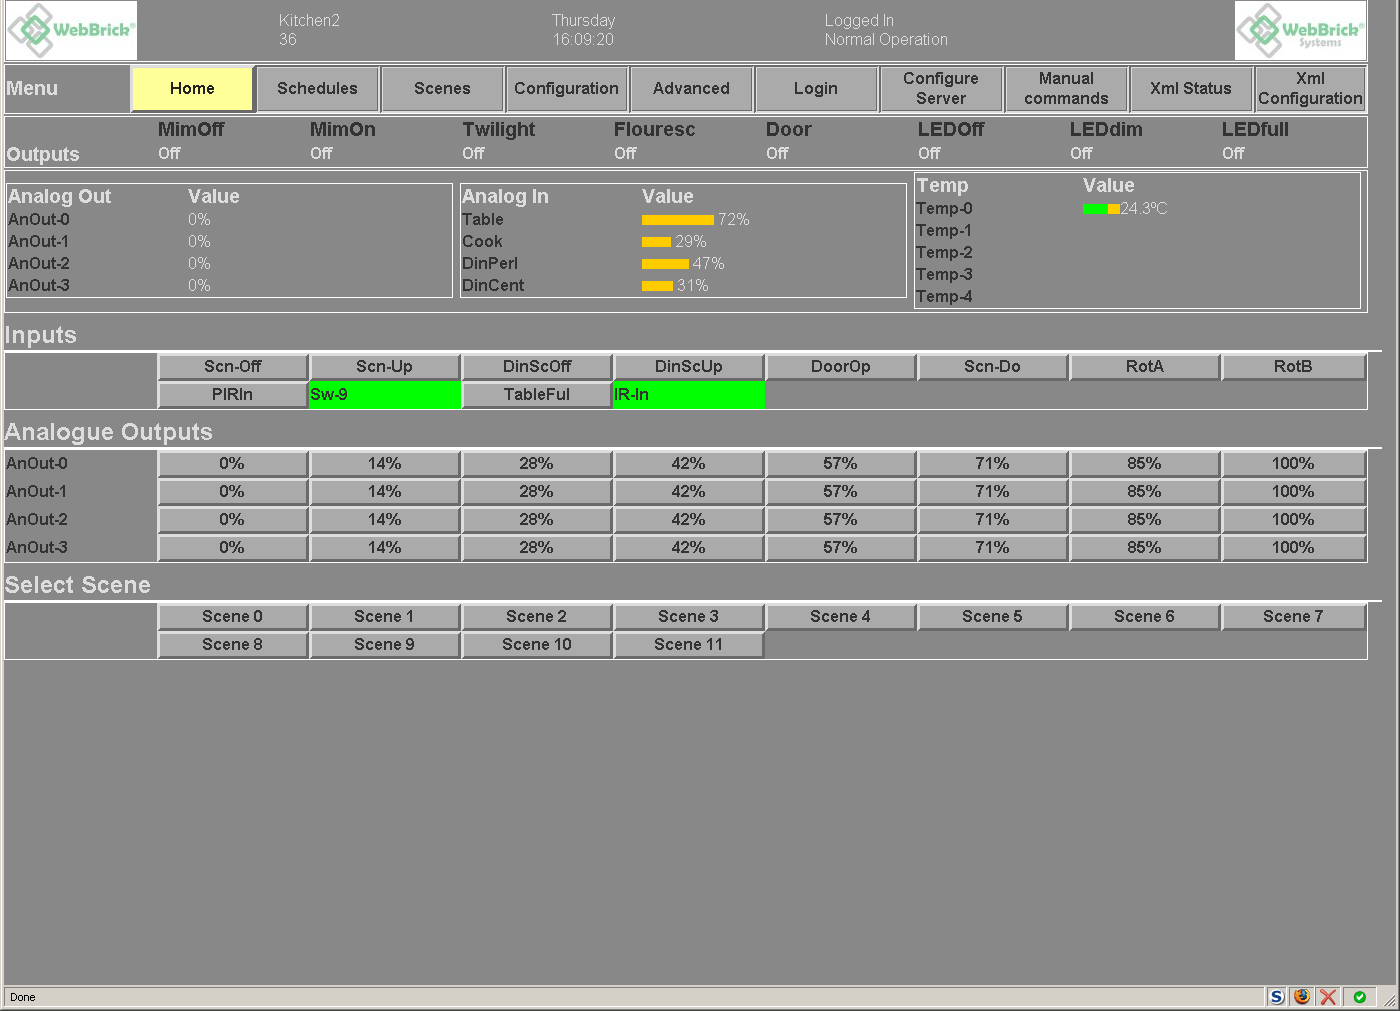
\includegraphics[width=0.9\textwidth]{Images/home.png}
\caption{Example of WebBrick Home Page}
\end{figure}
\subsection {History}

\index{History of WebBrick}

WebBrick started life as a bespoke project and in that incarnation there are 50-100 of them installed handling
tasks from building security to heating control, the largest setup uses 75+ WebBrick to manage a single house.
The latest incarnations (WebBrick6 and the WebBrick 7 Series) is a commercial project with added facilities.
The V6 WebBrick has an added IO board which provides screw terminals for all connections. It also has 4 Mains switching 
triacs and 2 Double pole changeover relays as well. We can also produce bespoke versions of the IO board
for specific uses.


\subsection {7 Series WebBrick}

The V6.4 WebBrick has the following connections:

\index{connections}

\begin{enumerate}

\item
8 Digital Outputs available as a combination of TTL and Open Collector drives.

In the default configuration 4 digital outputs are connected to mains triacs and can handle up to 500W 
per channel with a maximum of 1500W across all 4 channels. 2 of the Open collector outputs are connected to double pole 
changeover relays. 4 channels are available as TTL outputs.

The open collectors can sink to ground 3A, note that this was previously 500mA on the 6 Series

Digital Out 7 (TTL) can drive RC5 IR sequences to a suitable IR LED.

\item
8 Mimic outputs.  These are available at TTL and 12V levels are used to indicate the state of the WebBrick outputs.
The main functions of these mimics is to drive indicator LEDs found on push buttons. They are PWM modulated so that the
brightness can be modified for the on and off phases. The internal analogue and digital outputs can be configured to set 
the mimics to the on or off brightness(0..63) levels or they can be directly controlled from a system external to the WebBrick.

\item
12 Digital Trigger Inputs, TTL level - These can be treated as de-bounced push-buttons or toggle [MK] style inputs.  
The actual trigger point can be the rising edge, falling edge or both. When used in adjacent even/odd pairing Digital inputs will support 
rotary encoders.

All inputs have weak pullups so that switches can be connected with no further components involved.

Digital Input 11 can be configured to accept RC5 IR commands when connected to a suitable sensor.

\item
4 Analogue Outputs 0-10V. When the output level is changed, a new target value is set, these outputs 
adjust the output value over a time period (Fade Rate). Fade Rate is adjustable and can be as short as 200mS for full range 
change or as long as 50 Seconds.

\item
4 Analogue Inputs These are 0-5V input, high impedance - 47K, care must be taken not to exceed 5V on this pin, 
the web interface displays 0-100.

\item
One Wire Bus for up to 5 off Dallas DS18B20 temperature sensors.  On the 7 series the 5V supply and ground are specifically for temperature and humidity sensors.  The 5V supply is is specially decoupled and is limited to 10mA.  As a historical note this change was made to protect the WebBricks from shorts or excessive noise on sensors lines.

\item
RJ45 connection for 10Mb/s Ethernet.

\item
Serial output that can be configured for RS232, RS485 or DMX protocols.

\item
12V power connection

\end{enumerate}



\subsection {The Version 6.4 WebBrick}

The V6.4 WebBrick has the following connections:

\index{connections}

\begin{enumerate}

\item
8 Digital Outputs available as a combination of TTL and Open Collector drives, with an option for 8 more on bespoke 
developments. 
In the default configuration 4 digital outputs are connected to mains triacs and can handle up to 500W 
per channel with a maximum of 1500W across all 4 channels. 2 Of the Open collector outputs are connected to double pole 
changeover relays. 4 channels are available as TTL outputs.

\item
8 Mimic outputs.  These are available at TTL level are used to indicate the state of the WebBrick outputs.
The main functions of these mimics is to drive indicator LEDs found on push buttons. They are PWM modulated so that the
brightness can be modified for the on and off phases. The internal analogue and digital outputs can be configured to set 
the mimics to the on or off brightness(xx) levels or they can be directly controlled from a system external to the WebBrick.

\item
12 Digital Trigger Inputs, TTL level - These can be treated as de-bounced push-buttons or toggle [MK] style inputs.  
The actual trigger point can be the rising edge, falling edge or both. All inputs have weak pullups so that 
switches can be connected with no further components involved.

\item
4 Analogue Outputs 0-10V. When the output level is changed, a new target value is set, these outputs 
adjust the output value over a time period (Fade Rate). Fade Rate is adjustable and can be as short as 200mS for full range 
change or as long as 50 Seconds.

\item
4 Analogue Inputs This is a 0-5V input, high impedance, care must be taken not to exceed 5V on this pin, 
the web interface displays 0-100.

\item
One Wire Bus for up to 5 off Dallas DS18B20 temperature sensors.

\item
RJ45 connection for 10Mb/s Ethernet

\item
12V power connection

\end{enumerate}

Note that the Rotary Encoder connections from the pre 6.2 WebBrick have been incorporated into standard Digital Inputs, up to
6 rotary encoders can be supported.
